\documentclass[aspectratio=169]{beamer}
% Optional: Customize Beamer theme and colortheme here if desired.
% If none specified, mucomp defaults to the Pittsburgh theme with beaver colortheme.
% \usetheme{Madrid}
% \usetheme{AnnArbor} \usecolortheme{wolverine}
% \usetheme{CambridgeUS}
% \usetheme{Frankfurt} \usecolortheme{seahorse}
% \usetheme{Warsaw}
\usepackage{mucomp}

% Add bibliography resource
\addbibresource{references.bib}

\title{Computational Methods in Relativistic Hydrodynamics}
\subtitle{Applications to Astrophysical Mergers and Explosions}
\author[Biswas]{Biswarup Biswas}
\coauthors{the MU Computational Maths Group}
\institute[MU]{Department of Mathematics, Mahindra University}
\conference{National Conference on Computational Mathematics}
\minisymposium{Special Session on Numerical Relativity}
\date{\today}
\titlegraphic{
\includegraphics[height=1.0cm]{MU_logo.png}}
\logo{
\includegraphics[height=0.45cm]{MU_logo.png}}

\begin{document}

\begin{frame}[plain]
  \titlepage
\end{frame}

\begin{frame}{Introduction to Relativistic Gases}
  \begin{itemize}
    \item Relativistic hydrodynamics (RHD) plays a crucial role in modeling high-energy astrophysical phenomena.
    \item Examples include binary neutron star mergers\fcite{baiotti2017binary}.
    \item The thermodynamic properties of a relativistic gas are often modeled using the Synge equation of state\fcite{synge1958relativistic}.
    \item In extreme gravitational fields, we rely on Einstein's field equations to describe BNS mergers\fcite{baiotti2017binary}.
  \end{itemize}
\end{frame}

\section{Numerical Methods}

\begin{frame}{Mathematical Formulations}
  \begin{theorem}[Conservation Laws]
    The governing equations of relativistic hydrodynamics can be written as a system of hyperbolic conservation laws:
    \[
      \frac{\partial \mathbf{U}}{\partial t} + \sum_{i=1}^3 \frac{\partial \mathbf{F}^i(\mathbf{U})}{\partial x^i} = \mathbf{S}(\mathbf{U})
    \]
    where $\mathbf{U}$ is the vector of conserved variables.
  \end{theorem}
  
  \begin{definition}[Primitive Variables]
    The primitive variables (e.g., density $\rho$, velocity $\mathbf{v}$, and pressure $p$) must be recovered from the conserved variables $\mathbf{U}$ at each time step, typically requiring numerical root-finding methods.
  \end{definition}
\end{frame}

\section{Simulation \& Visualization}

\begin{frame}{Simulation of 2D Relativistic Flows}
  \begin{columns}
    \begin{column}{0.45\textwidth}
      \textbf{Dynamics of RHD Shockwaves}
      \begin{itemize}
        \item Relativistic shockwaves exhibit complex interface instability.
        \item High-order WENO schemes are employed to resolve the shocks without spurious oscillations.
        \item The animation on the right shows the evolution of the density field over 21 frames.
      \end{itemize}
    \end{column}
    \begin{column}{0.45\textwidth}
      % Demonstration of the PDF animation helper \pdfanim
      % Usage: \pdfanim[options]{prefix}{first}{last}
      \centering
      \pdfanim[width=\textwidth,fps=5,loop=true,autoplay=true]{RP2D1_frames/frame_}{0001}{0021}
      \vskip0.5em
      \scriptsize{Figure: 2D Relativistic flow evolution.}
    \end{column}
  \end{columns}
\end{frame}

\begin{frame}{Embedded Video: WENO Simulation}
  \begin{columns}
    \begin{column}{0.45\textwidth}
      \textbf{KPP 2D WENO Simulation}
      \begin{itemize}
        \item This slide displays the compiled MP4 video directly.
        \item The simulation models 2D wave propagation using high-order WENO schemes.
        \item Click on the placeholder image on the right to start playing the video.
      \end{itemize}
    \end{column}
    \begin{column}{0.55\textwidth}
      \centering
      \embedmpfour[width=0.6\textheight,height=0.6\textheight]{%
        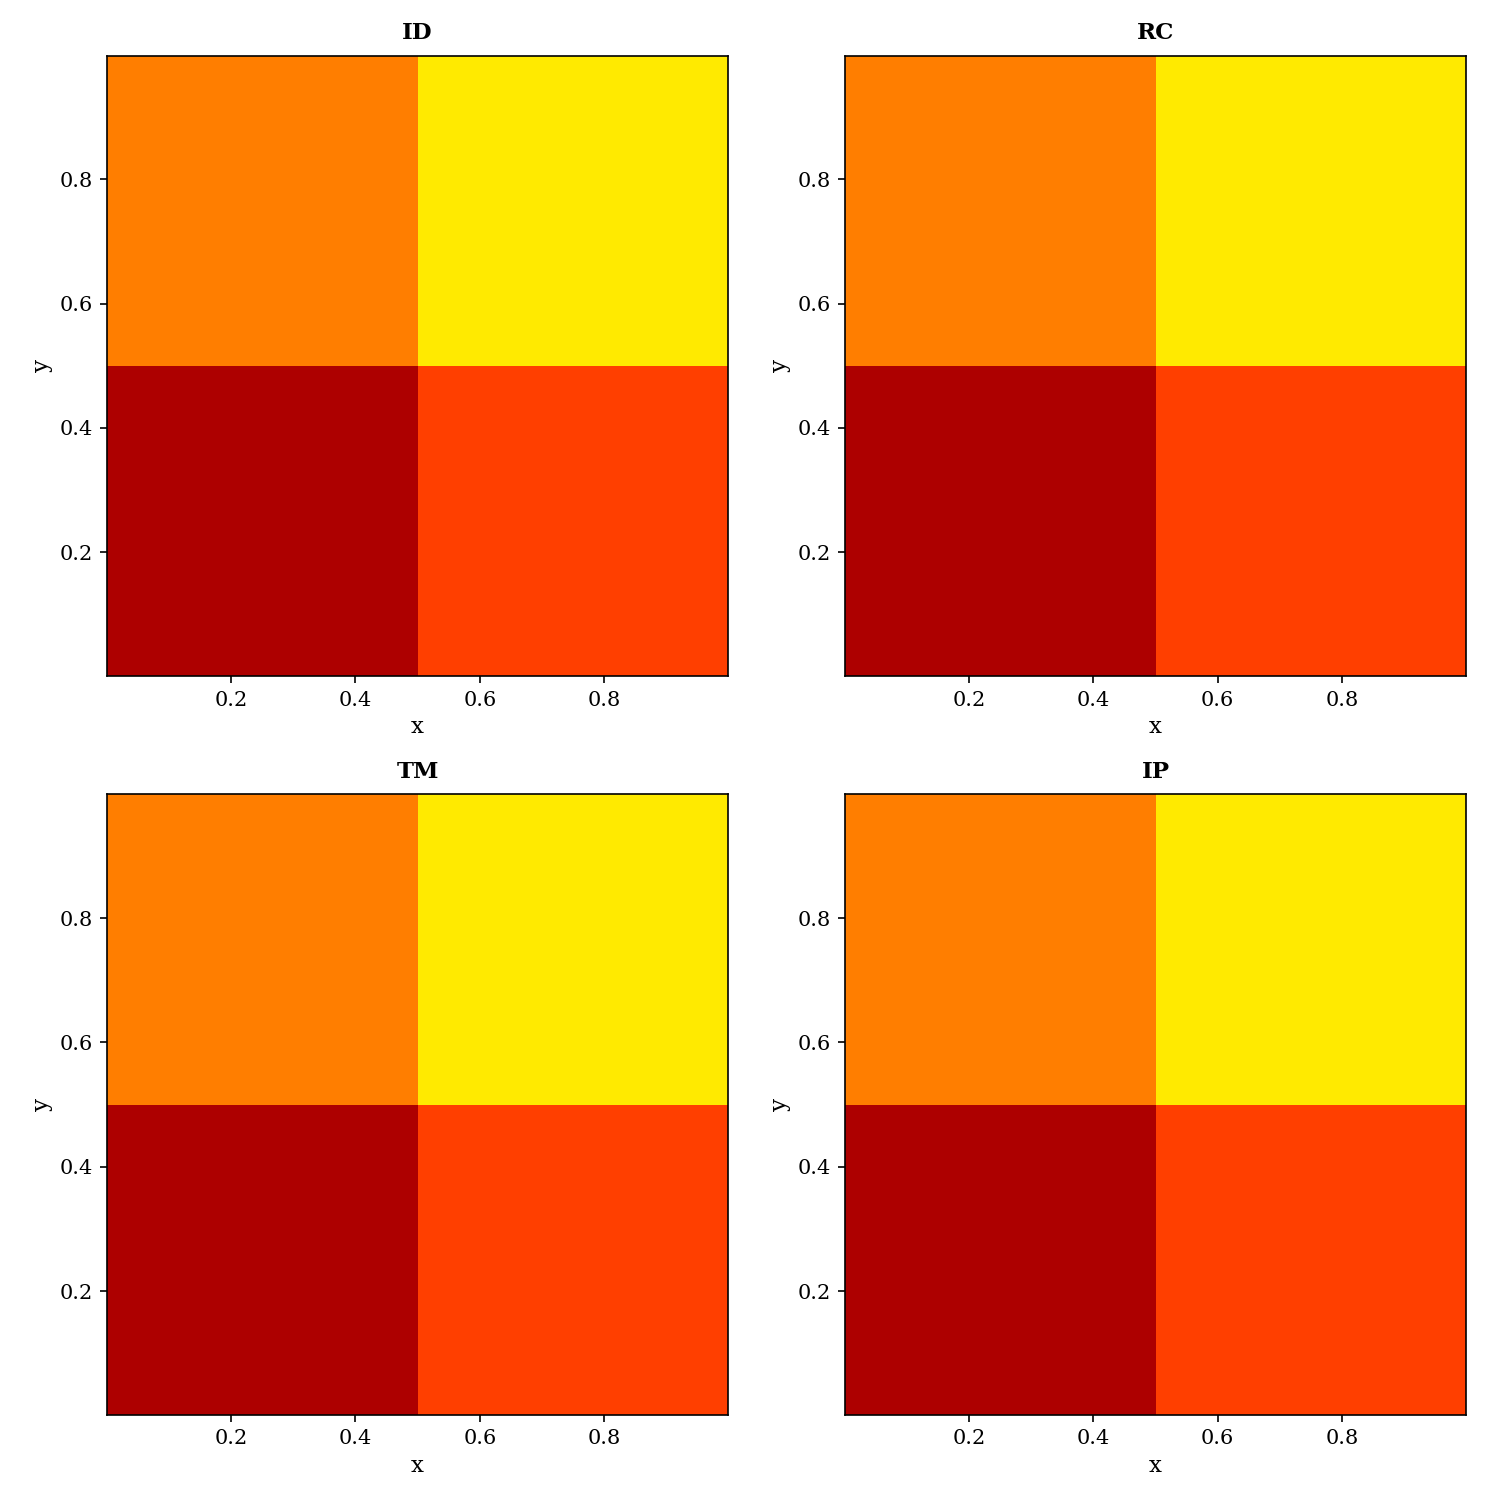
\includegraphics[width=0.6\textheight,height=0.6\textheight]{RP2D1_frames/frame_0001.png}%
      }{KPP_2D_WENO.mp4}


      \vskip0.5em
      \scriptsize{Video: 2D Relativistic simulation (click to play).}
    \end{column}
  \end{columns}
\end{frame}

\begin{frame}{Conclusion}
  \begin{itemize}
    \item Robust numerical schemes are essential for simulating relativistic flows.
    \item The \texttt{mucomp} package provides support for standard theme styles, math blocks, footnoting/citations, and animations.
  \end{itemize}
\end{frame}

\end{document}
